% tags: blockDiagram doubleArrow fit variable arrowHead triangleArrowHead
% postaction postAction triangle
\PassOptionsToPackage{usenames,dvipsnames}{xcolor}
\documentclass[tikz,border=2]{standalone}
%%\usepackage{gillius2}
%%\renewcommand{\familydefault}{\sfdefault}
\usepackage{lmodern} % enhanced version of computer modern
\usepackage[T1]{fontenc} % for hyphenated characters and textsc in section title
\usepackage{amssymb}
\usepackage{enumitem}
\usepackage{mathtools} % contains amsmath which comes with align
\usepackage{amsthm}
\usepackage{graphicx}
\usepackage{microtype} % some compression
\usepackage[skins]{tcolorbox}
%%%%%%%%%%
% brown blue red
\definecolor{LightBlue}{HTML}{C7DFE3}
\definecolor{DarkBlue}{HTML}{72AFB6}
\definecolor{DarkBrown}{HTML}{D2BE89}
\definecolor{LightBrown}{HTML}{F4ECDF}
\definecolor{Grey}{HTML}{A7A195}
\definecolor{Red}{HTML}{CA6C2E}
%%
\def\labelitemi{\textcolor{gray}{\tiny{$\blacksquare$}}}
\def\labelitemii{\textcolor{gray}{\tiny{$\square$}}}
\setlist{itemsep=-1ex,leftmargin=*}
%%%%%%%%%%%%%%%%%%%%%%%%%%%%%%%%%%%%%%%
% Define the layers to draw the diagram
%%
\usetikzlibrary{shadows,arrows,shapes,positioning,calc,backgrounds,
fit,automata,decorations.markings,
decorations.pathreplacing,decorations.pathmorphing}
%%%%%%%%%%%%%%%%%%%%%%%
\def\ps{4cm}
\begin{document}
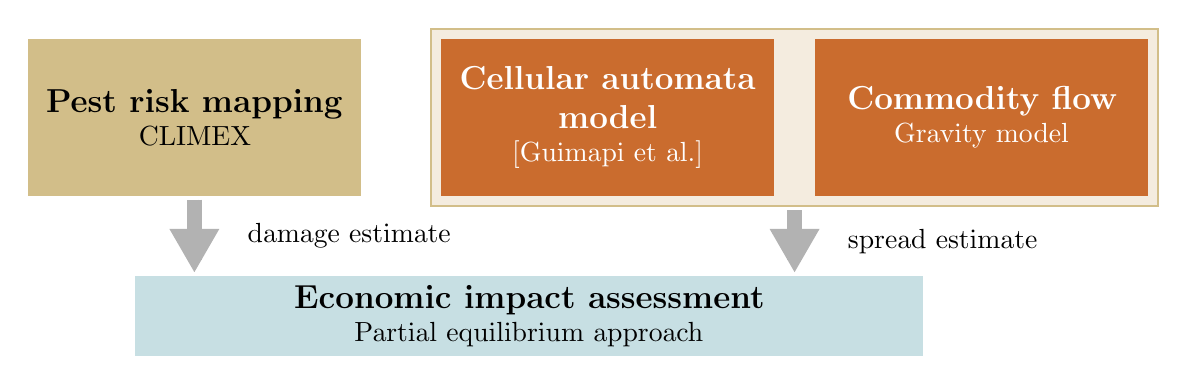
\begin{tikzpicture}
[scale=1,auto, transform shape,
   block/.style={font=\large\bf,rectangle,minimum height=2cm,minimum
   width=4cm,text=black,fill=black!20},
   lb/.style={text=black},
regedge/.style={gray!60,>=triangle 60, shorten >=.4mm, shorten <=.4mm, 
line width=1.2mm,postaction={draw, line width=2mm, shorten >=2mm, -}}]
\node[block,fill=DarkBrown] (climex) {\parbox{\ps}{\centering Pest risk
mapping\\\normalsize\normalfont CLIMEX}};
\node[block,text=white,fill=Red,right=of climex] (ca) {\parbox{\ps}{\centering Cellular
automata model\\\normalsize\normalfont [Guimapi et al.]}};
\node[block,text=white,fill=Red,right=of ca,shift={(-.5cm,0)}] (gravity) {\parbox{\ps}{\centering Commodity
flow\\\normalfont\normalsize Gravity model}};

\begin{pgfonlayer}{background}
   \node[fit=(ca)(gravity),thick,rectangle,draw=DarkBrown,fill=LightBrown] (spread) {};
\end{pgfonlayer}

\node[block,fill=LightBlue,below=of ca,minimum height=1cm,minimum
width=10cm,shift={(-1cm,0)}] (econ) {\parbox{7.8cm}{\centering Economic impact
assessment\\\normalsize\normalfont Partial equilibrium approach}};
\draw[regedge,->] (climex.south) -- (econ.north -| climex.south)
node[lb,midway,shift={(.5cm,0)}] {damage estimate};
\draw[regedge,->] (spread.south) -- (econ.north -| spread.south)
node[lb,midway,shift={(.5cm,0)}] {spread estimate};
%%
\end{tikzpicture}
\end{document}

